\documentclass[a4paper]{article}
\usepackage{amsmath}
\usepackage{graphicx}
\usepackage[margin=1in]{geometry}
\usepackage{setspace}
\usepackage{subfigure}
\usepackage{multirow}
\usepackage{caption}
\usepackage[table]{xcolor}
\linespread{1.2}
\rowcolors{1}{blue!20}{blue!10}
\newcommand{\tabincell}[2]{\begin{tabular}{@{}#1@{}}#2\end{tabular}}
\begin{document}
\section{Question 1}
~~~~The question is to write a function, where we provide :~ 1.The interpolation points-values pairs~2.The evaluation points. Then the function can return the vector containing the values that the interpolation polynomial take at the evaluation points.\\
\indent For interpolation, we use Lagrange Interpolation. To construct the polynomial verbally, we need to observe the structure. Lagrange polynomial is nothing but a linear combination of n polynomials. So we can use a double iteration to construct it.\\
\textbf{function: Lagarange\_interpolation}\\
\indent For the external interpolation, we use $j$ to track the number of the element polynomial that we are at. At each stage, we fix the external iteration cursor $j$, and construct the corresponding element polynomial using a internal iteration. Using a subscript $k$ to iterate through all of the input points except $j$, we calculate the cumulative product $\prod_{k\neq j}\frac{x-x_k}{x_j-x_k}$. Then multiply it by the coefficient $f(x_j)$, and add it to the total sum, which is initially set to 0.\\
\textbf{function: output1}\\
\indent Now we've successfully constructed a function to evaluate a Lagrange Interpolation at single point, we just need to iter through all the evaluation points to get the whole output vector, then it's done.
\textbf{function: main function}\\
\indent After developing the output function, we get to test the evaluation using two kind of interpolating points: the uniform version and the Chebyshev version. It is nothing but using linspace function to generate them and pass it to the output function.
\section{Question 2}
~~~~The question ask us to do the same thing as in question 1, but this time we change the method of interpolating, to barycentric interpolation. To implement this, we still us a double iteration\\
\textbf{function: barycentric\_interpolation}\\
\indent For the external interpolation, we still, use $j$ to track the number, but now we need track the numerator and the denominator simultaneously because they both iterate through all of the interpolation points. For each fixed $j$ we adopt a internal iteration to construct the $\lambda_j$, we iter through all points but the one that $k=j$, and calculate the cumulative product $\frac{1}{\prod_{k\neq j}(x_j-x_k)}$. Then add the proper expression to numerator and denominator. After all iteration, we divide the numerator by denominator and get the result.\\
\textbf{function: output2}\\
\indent Now we've successfully constructed a function to evaluate a Barycentric Interpolation at single point, we just need to iter through all the evaluation points to get the whole output vector, then it's done.
\section{figures output}
\begin{figure}[!ht]
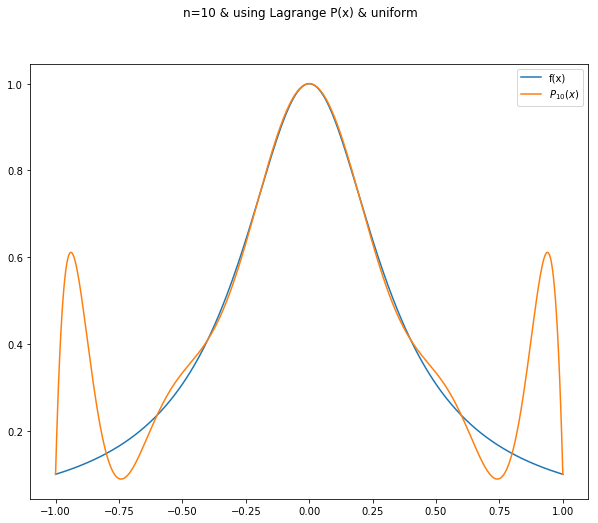
\includegraphics[scale=0.5]{10&u.png}
\end{figure}
\begin{figure}[!ht]
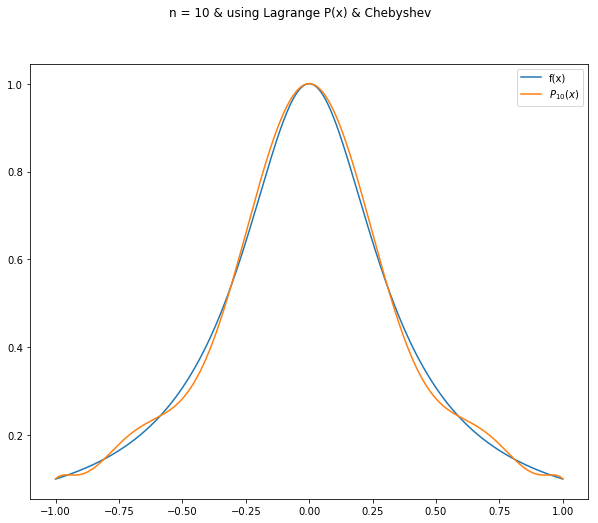
\includegraphics[scale=0.5]{10&C.png}
\end{figure}
\begin{figure}[!ht]
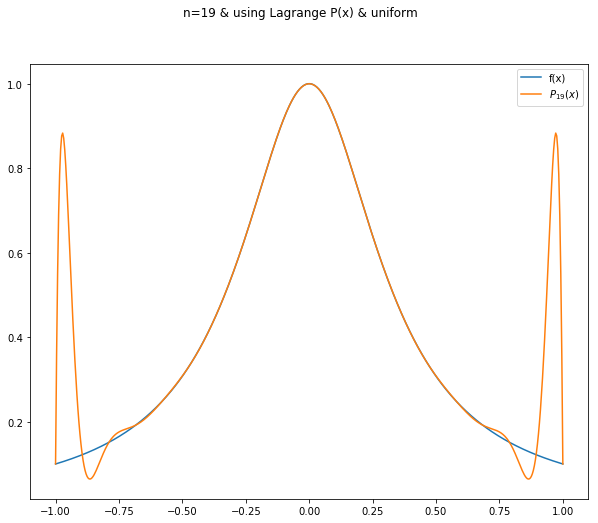
\includegraphics[scale=0.5]{19&u.png}
\end{figure}
\begin{figure}[!ht]
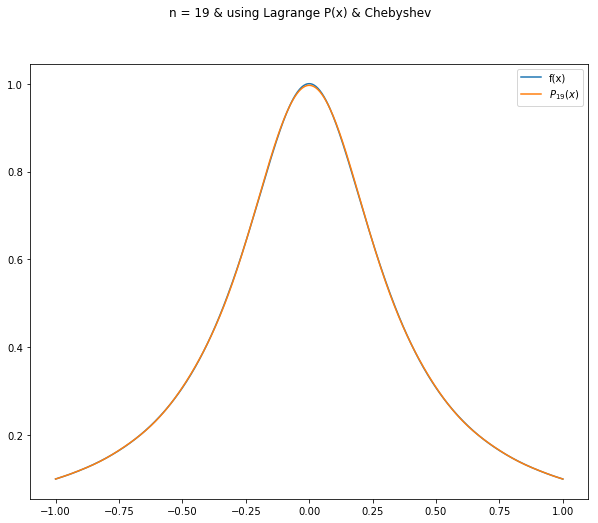
\includegraphics[scale=0.5]{19&C.png}
\end{figure}
\begin{figure}[!ht]
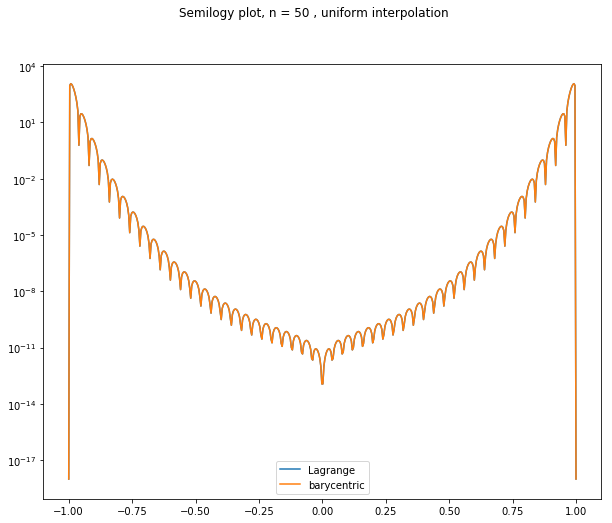
\includegraphics[scale=0.5]{50&U.png}
\end{figure}
\begin{figure}[!ht]
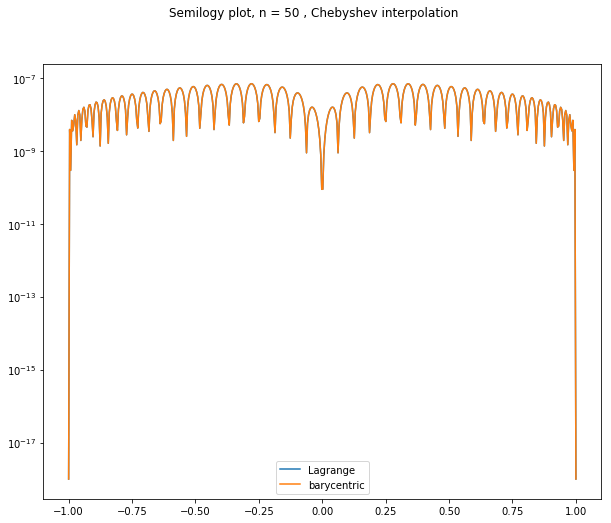
\includegraphics[scale=0.5]{50&C.png}
\end{figure}
\begin{figure}[!ht]
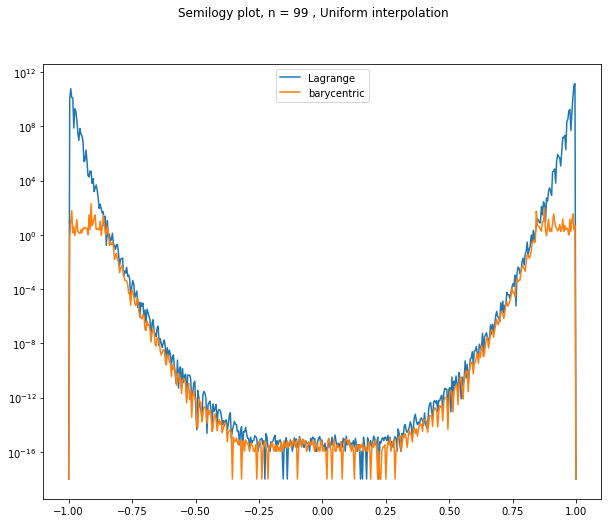
\includegraphics[scale=0.5]{99&U.png}
\end{figure}
\begin{figure}[!ht]
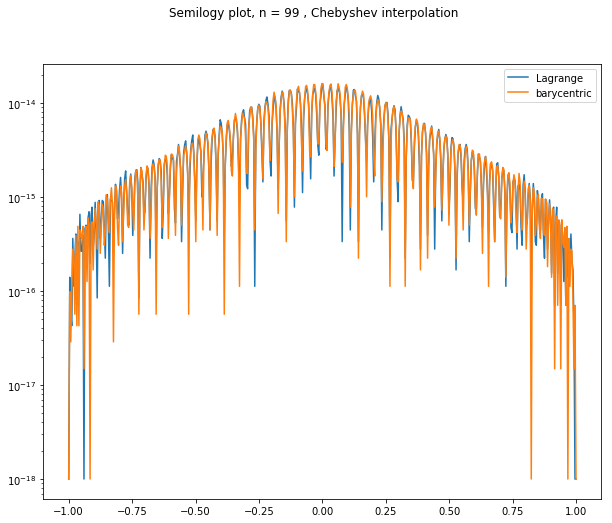
\includegraphics[scale=0.5]{99&C.png}
\end{figure}
\section{Comments on the figures}
\subsection{Comments on the first 4 figures}
We can observe from the first 4 figures that as the number of interpolating points increase, the accuracy of interpolation is increasing. But if we are using a uniform grid, there is a sharper and sharper deviation in the two tails of the interpolating interval. Using the Chebyshev interpolation can overcome this draw back. After adopting the Chebyshev grid, the interpolation polynomial tends to converge to the original function over whole interpolation interval.
\subsection{Comments on the last 4 figures}
These figures are about the error of the interpolating. We can see that using uniform grid ,the error is smaller in the middle and larger in the tails. And the error in the tails can be much smaller if we are using barycentric interpolation. If we are using Chebyshev grid, the error is relatively large in the middle and small in the tail, but overall, they are much smaller than the error of using the uniform grid.
\end{document}
